%!TEX root = ../../main.tex

\chapter{Fabrication of Nanodiamonds}	\label{ch::fabrication_nanodiamonds}
\chaptermark{Fabrication of Nanodiamonds}

	\begin{remark}
			\item die section mit den \si implanted \nds muss von dir ueberarbeitet werden. Die hab ich deshalb vorerst ausgelassen. Es gibt 3 teile (einfuehrung, preliminary tests und final procedure). Ich hab den eindruck, dass sich da konzeptionell vieles wiederholt und das man das ganze vielleicht in einer section unterbringen kann und die feineren unterscheidungen einfach beilaeufig erwaehnt.
			\item section iridium substrate sollte auch nochmal durchgelesen werden. Ich habs zwar nochmal ueberarbeitet, aber ich denke da koenntest du noch den einen oder anderen erklaerendne statz springen lassen. Insbesondere das listin in preparation of substrate ist nicht gerade selbsterklaerend.
			\item Die tabelle mit dem ueberblick ueber alle samples hab ich in eine eigene section geschoben. Die is ja wichtig, weil in den results immer wieder die sample id genannt werden. Wennd as im inhaltsverzeichnis auscheint, find ich das praktisch.
	\end{remark}

	\epigraph{``Diamond forms under high temperature and pressure conditions that exist only about 100 miles beneath the earth's surface.''}{\textup{Gemological Institute of America Inc.}}

	Due to its extraordinary properties, diamond has transcended its sole purpose as a rare gem and developed into an important tool enabling various applications in industry and research. This change has been driven largely by the development of methods allowing to cheaply produce synthetic diamond. While synthetic diamonds are typically small and without the splendeur generally associated with diamond, they can be produced on-demand and are thus arguably more useful than rare gemstones.
	In this chapter we introduce the two most common methods for the fabrication of diamonds in a laboratory setting: The \hpht and the \cvd method.
	The aptly named \hpht (\HPHT) process mimics the conditions under which diamond is formed in nature and is widely used to synthetically produce diamonds for industrial applications such as utilization of diamond as a abrasive.
	While \HPHT diamonds are utilized in this work, most reported measurements are based on diamond produced with the \CVD method in which diamonds are grown using a hydrocarbon gas mixture. Both processes have incommon that defects and impurities are a naturally occuring.
	For a more extensive list of diamond production processes refer to \cite{davis1993diamond}.
	In the context of this thesis nano-sized dimonds are required. They can be obtained by milling larger sized \HPHT or \CVD diamonds down to the desired grain size in a vibrational mill.
	The obtained \nds are small enough that individual specimen have a chance of hosting a singleton \siv. These can be identified and used for further exploration.

\section[HPHT]{High-Pressure High-Temperature Diamond}\label{sec::hpht}

	The \HPHT method was the first process to successfully synthesize diamond in 1879.
	Today, it is still widely used due to its relatively cheap production costs for small diamonds \cite{wikiSyntheticDiamond}.
	\\
	In the \HPHT process, diamond is synthesized from graphite under temperatures of up to \SI{1.5d3}{\celsius} pressures between \SI{5d4}{bar} and \SI{d6}{bar} \cite{davis1993diamond}. Under these extreme conditions, carbon transitions from its graphite to its diamond phase because the latter becomes energetically favorable \cite{janine::135, janine::136, janine::137, janine::138}.
	The machine used for this kind of synthesis is a press.
	For some forms of this method, a metallic catalyst solvent is added lowering the required pressures and temperatures by causing graphite to dissolve earlier. At the same the catalyst promotes the crystallisation process.
	Several press designs exist, all of which relying on creating and maintaining high pressures and a high temperatures.
	While it is possible to grow big ($> \SI{10}{\carat}$) high-quality diamonds with the \HPHT process, its cost quickly increases and thus becomes unfavorable.
	\\
	In this thesis, \HPHT \nds diamonds produced by Davydov et al. \cite{Davydov2014} are spectroscopically investigated.


\section[CVD]{Chemical Vapor Deposition Diamond}\label{sec::cvd}




	In contrast to the \HPHT method, diamond is crystallized from carbon available in the gas phase in the \CVD method.
	The process still requires respectable temperatures in the range of \SIrange{700}{1300}{\celsius} but makes due with the low pressures of less than \SI{1}{\bar} available in a vacuum growth chamber \cite{janine::141}.

	The chamber contains a vapour consisting of a mixture of atomic hydrogen and methan. The gas can be forced into the plasma phase using strong microwaves or hot filaments \cite{neu::75, neu::78, neu::79}. While the hot filament is easy to implement, it has the disadvantage that atoms which are etched from the filament during the growth process are likely to contaminate the diamond. To minimize the introduction of defects other than \sivs in the diamond, growing diamonds in a microwave plasma is preferred. In it methane molecules dissociate and relase carbon. In the presence of a substrate such as \ir containing suitable seeds, carbon can crystalize forming diamond. \autoref{fig::cvd_sketch} illustrates the setup. In a plasma containing atomic hydrogen, the formation of diamond is favored over the formation of graphite. This is due to the fact that the atomic hydrogen preferentially etches $sp2$ bonded carbon, i.e.\ graphite.

	\begin{figure}[htp]
		\centering
		\testbox{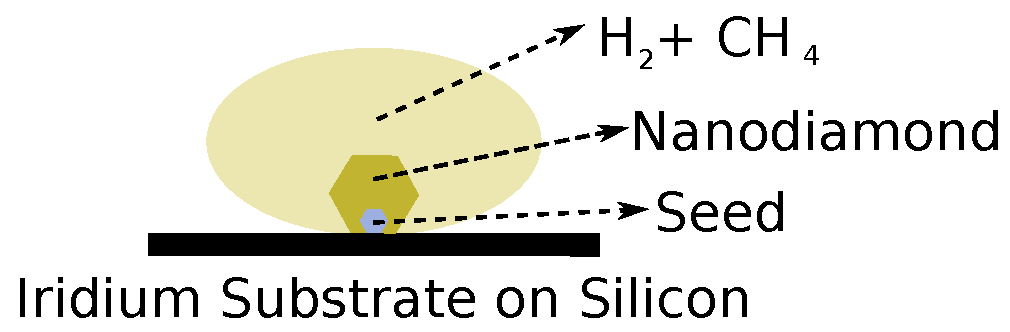
\includegraphics[trim = 0 0 0 0,  clip= true, width = 0.3\textwidth]{./pics/cvd_sketch.pdf}}
		\caption[\CVD production method]{Sketch of the \CVD method. A hydrogen-carbon plasma acts as a donor for carbon atoms which may crystalize to form diamond ontop of a suitable \ir substrate. An initial diamond seed facilitates the process.}
		\label{fig::cvd_sketch}
	\end{figure}

	Typically, single crystal diamond substrates are required to grow single crystal diamond. \HPHT substrates are suitable to start a crystalization process. This approach is referred to as homoepitaxial growth. An alternative approach is to utilize non-diamond substrates such as \ir or platinum to trigger heteroepitaxial growth \cite{janine::142, neu::143}.
	This method is utilized for all the \CVD \nds grown and investigated in this thesis.
	It relies on small diamond crystals deposited in the substracte acting as seeds for the diamond crystalization process. Seed diamond crystals are commercially available, and are usually particles produced by a so-called detonation process.
	In a detonation process, the high pressure produced by shockwaves of a detonation is used to create very small diamond particles of a size down to a few nanometers.

	Growth on a substrate is favored, if the lattice constant of the substrate and the diamond to be grown are similar.
	The lattice constant of \ir is \SI{0.384}{nm} \cite{Arblaster2010,Gsell2007} and thus close to the lattice constant of diamond with \SI{0.356}{nm} \cite{Davis1993}.
	Therefore, we opted to grow diamond on a stratified substrate, consisting of \ir layers of \SIrange{60}{150}{nm} thickness. The \ir layers themselves were grown onto an yttria-stabilized zirconia (YSZ) buffer layer, which in turn was grown on a silicon wafer \cite{Gsell2004a}.
	If the lattice constant of the substrate and the diamond are not matched, stress in the diamond lattice is induced.
	Therefore, the \ir substrate not only facilitates diamond growth, but also reduces unfavorable stress in the \nds. The detremental effects of stress on the diamond lattice and its implications with respect to hosted \sivs are briefly discussed in \autoref{ch::distribution}.
	\\
	To produce \nds of controlled size, the growth process is stopped when the diamonds grown onto the seed crystals are large enough.
	If the growth process is continued, the individual crystals grow together to form diamond films.
	Such diamond films are used as starting material for the wet-milling process described in \autoref{sec::wet_milled_nds}.
	\\
	One of the advantages of the \CVD process is that \si is incorporated automatically into diamonds, \sivs can thus be formed \textit{in-situ} as the diamond is grown. The presence of \si atoms required to be absorbed into the diamond lattice is explained by the plasma etching the edges of the \si waver underneath the growth substrate.
	To further increase the \si content in the chamber, sacrificial \si can be introduced.
	\\
	After \nd growth, the \nds are either investigated directly on the growth substrate or transferred to an ultrasonic bath to obtain a solution which is coated onto other substrates for further exporation.
	\\
	In this thesis, two types of \nds samples were investigated.
	The first batch, henceforth referred to as \CVD samples, was grown by the group of \schreck using detonation diamond seeds of a size smaller than \SI{3}{nm}(produced by the company Microdiamant, product Liquid Diamond monocrystalline, MSY {0-0.03} micron GAF).
	For the growth process, \SI{1}{\percent} of methane was added to the hydrogen environment in the growth chamber.
	The growth process was performed with a pressure of \SI{30}{hPa} for \SIrange{30}{60}{min}, yielding \nds of a diameter of about \SIrange{100}{200}{nm}. A sample of the produced diamonds is given in \autoref{fig::sem_cvd}.

	\begin{figure}[htp]
		\begin{subfigure}[t]{ 0.49\linewidth}
			\caption{}\label{subfig::cvd_large}
			\centering
			\testbox{\includegraphics[trim = 0 0 0 0,  clip= true, height=5cm]{./pics/M05-13_191_131209_06.png}}
			% \caption{SEM picture of the milled nanodiamonds of a mean diameter of \SI{100}{\nano\meter}}
		\end{subfigure}
		\hfill
		\begin{subfigure}[t]{ 0.49\linewidth}
			\caption{}\label{subfig::cvd_detail}
			\centering
			\testbox{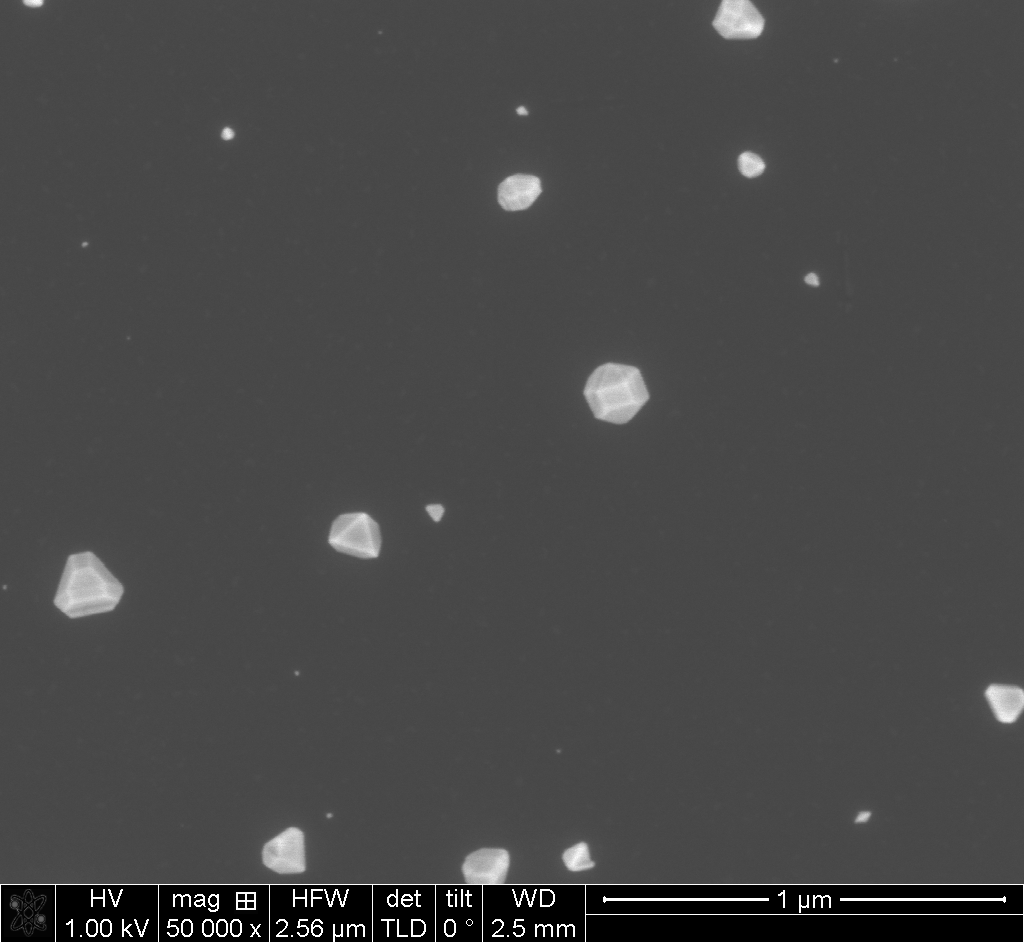
\includegraphics[trim = 0 0 0 0,  clip= true, height=5cm]{./pics/M05-13_191_131209_05.png}}
			% \caption{TEM picture of a \SI{100}{\nano\meter} diamond crystal.}
		\end{subfigure}
		\caption[Example of \CVD \nds]{SEM images of \CVD diamonds (sample \insitucvd) produced by M.\ Schreck's group at Augsburg University. The average size of these \nds is \SI{100}{nm}. (a) Overview image, white dots are \nds. (b) Detail image, it can be seen that \nd shape and size is varied.}
		\label{fig::sem_cvd}
	\end{figure}

	The second type of samples consist of \CVD \nds grown onto molecular analogs of diamond crystals.
	A subgroup of these molecular diamonds are called diamondoids and are carbon crystals based on the carbon cage molecule adamantane \ch{C10H16}.
	The molecular diamonds used for this work are adamantane in cyclohexane, mercapto adamantane in cyclohexane, and cyclohexane.
	Each of these seed crystals was used in different growth processes.
	During the growth process, either \SI{1}{\percent} or \SI{3}{\percent} methane was added to the hydrogen plasma and either \si (\ch{Si}) or \si dioxide (\ch{SiO2}) was injected to promote the formation of \textit{in-situ} incorporated \sivs, see \autoref{tab::diamondiods}.


	\begin{table}[htp]
		\centering
		\caption[Samples grown with diamondoid seeds]{Summary of the samples grown on diamondoid seed crystals.} \label{tab::diamondiods}
			\begin{tabular}{llll}
			\toprule
			Sample name & Seed crystals & Methane conc. & \Si source \\
			\midrule
			160211\_E & Mercapto adamentane in cyclohexane & 1\% & \ch{SiO2} \\
			160211\_F & Cyclohexane                        & 1\% & \ch{SiO2} \\
			160212\_C & Cyclohexane                        & 3\% & \ch{Si}        \\
			160212\_D & Adamentane in cyclohexane          & 3\% & \ch{SiO2} \\
			160212\_E & Mercapto adamentane in cyclohexane & 3\% & \ch{SiOs} \\
			160212\_F & Cyclohexane                        & 3\% & \ch{SiO2}\\
			\bottomrule
			\end{tabular}
	\end{table}


\section[Wet-Milling]{Wet-Milled Nanodiamonds}\label{sec::wet_milled_nds}


	In addition to growing \nds of a specific size directly via a \CVD process, macroscopic diamond starting material can be crushed to obtain small diamond particles.
	In contrast to \nds directly grown by a \CVD process, the process is divided into two sub-processes:
	At first a macroscopic diamond is produced using one of the methods introduced in this chapter. Then macroscopic diamond is continuously milled into smaller diamond particles.

	The wet-milled \nds investigated in this thesis were kindly provided by \muzha. During the wet-milling process small metal beeds in an aqueous solution are driven by the vibrations of a vibrational mill. The moving beads continously collide with the present diamonds and thus keep breaking them into smaller and smaller particles. A sketch of the process is shown in \autoref{fig::sketch_milling}. Steel contamination introduced by the beads can be eliminated in a post-processing treatment with acid.

	\begin{figure}[htp]
		\centering
		\testbox{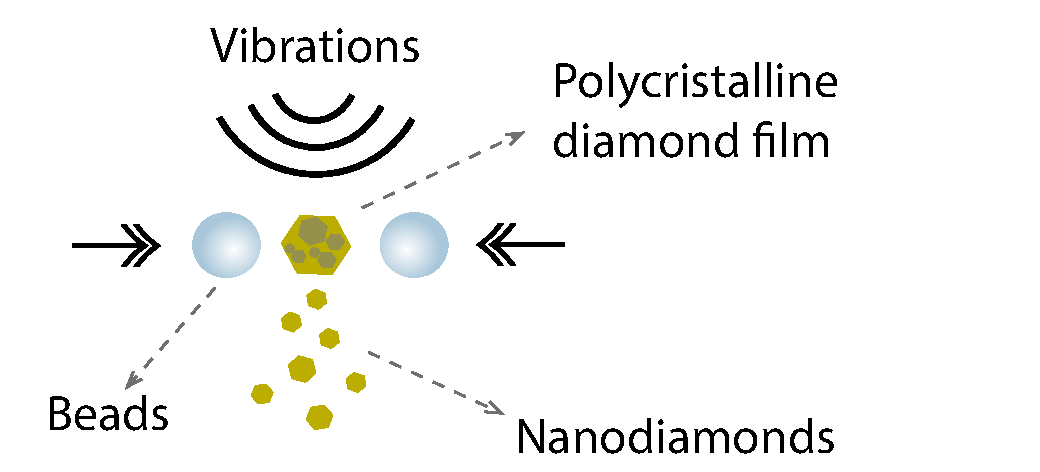
\includegraphics[trim = 0 0 0 0,  clip= true, width = 0.5\textwidth]{./pics/milling_sketch.pdf}}
		\caption[Wet-milling in a vibrational mill]{Sketch of a vibrational wet-mill. A macroscopic polycrystalline \nd is progressively broken down into smaller polycrystalline \nds by metal beads.}\label{subfig::sketch_milling}
	\end{figure}

	The big advantage of the milling process is that it enables the production of a large quantity of diamond nanoparticles.
	When producing \nds directly via a \CVD process, the number of produced \nds in one process scales with the surface of the substrate on which the \nds are grown.
	In contrast, the quantity of milled \nds scales with the volume of the starting material.
	Another advantage of the wet-milling process is that the \nds are alerady in an aqueous solution after milling.
	Therefore, it it can be used to spin-coat the \nds directly onto any substrate. Samples created in this fashion can directly be used for further investigation and do not require additional processing.
	\\
	If the starting material for the wet-milling process is a polycrystalline diamond film, it is likely to break along distinct crystal boundaries.
	However, due to imperfections in the growth process, particles may break down such that progressively smaller milled diamond grain remain polycrystalline.
	As a result, the final \nds contain crystal boundaries themselves, indicative of reduced crystal quality.
	To improve diamond quality \nds are treated with post-processing steps including annealing in vacuum and oxidation in air.
	A detailed description of these processes and their effects is given in \autoref{ch::crystal_quality}.
	\\
	In general any diamond, independent of production method, can be used as starting material for the milling process.
	In the following sections, avaiable sampels are distinguished by the respective staring material and milling method.

	\subsection{Wet-Milled \HPHT \Nds}\label{subsec::milled_hpht_nds}
		We investigated \nds wet-milled from a \HPHT starting material to median sizes of about \SIlist{45;80;260}{nm}.
		They were then drop-cast onto an \ir substrate and implanted with \ch{^{28}Si^1+} \todo[fancyline]{Complete implantation parameters}. The implantation itself was performed by \rogalla.
		% After impalntation, the \nds of a size of \SI{80}{nm} (sample \hphtimpeighty) were annealed in vacuum for \SI{1}{\hour} at \SI{1000}{\celsius}, \SI{900}{\celsius} for \SI{3}{\hour}.
		All \HPHT \nds were oxidized in air at \SI{450}{\celsius} for \SI{3}{\hour}. Resulting samples available for explorations are designated \hphtimpfortyfive, \hphtimpeighty, \hphtimptwosixty and listed in \autoref{tab::samplenames}.

	\subsection{Wet-Milled \CVD \Nds}\label{subsec::milled_nds}
		% - milled CVD diamond film (in-situ SiV)

		\begin{figure}[htp]
				\centering
				\testbox{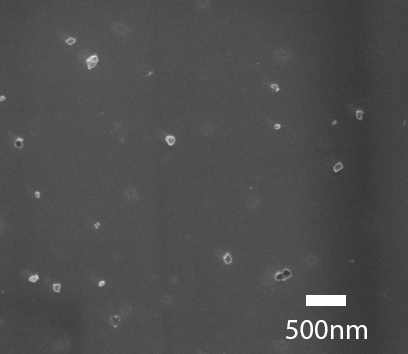
\includegraphics[trim = 0 0 0 0,  clip= true, height=5cm]{./pics/Ir27M_mitte_213_151111_22_crop.jpg}}
			\caption[Distribution of \nds ontop of an \ir substrate]{Pictures of milled \nds (sample \insituH) showing the distribution of the \nd crystals on the \ir substrate.}
			 \label{fig::sem_millling}
		\end{figure}

		In the following paragraphs, details of the production processes of \nd produced by wet-milling a \CVD diamond film in a vibrational mill are given.
		For an overview of the samples refer to \autoref{tab::samplenames}.
		The starting material for the wet-milled \nds was a nanocristalline diamond film \cite{Williams2006a} directly grown on a silicon wafer by \CVD.
		A microwave hydrogen plasma containing \SI{1}{\percent} methane was used to grow on purified \SI{5}{\nano\meter} nanodiamond seeds (produced by PlasmaChem).
		To induce \textit{in-situ} \siv creation, sacrificial \Si pieces are placed in the growth chamber.
		During diamond growth the \si pieces are etched by the plasma leading to individual atoms being incorporated into the diamond lattice.
		The diamond film is then wet-milled in a vibrational mill with steel beads.
		The high amount of steel containment due to the steel beads is removed by extensive acid treatment.
		We also investigated \nds milled with silicon nitride beads, and found that the choice of material of the beads does not result in any noticable difference in dependent measurements.
		The median diameters of the diamonds are \SIlist{50; 70; 100}{\nano\meter} as determined by laser diffraction spectroscopy. \autoref{subfig::sem_milled} shows milled \nds ontop of an \ir substrate.
		The aqueous solution containing the \nds is drop cast onto an \ir film on a \Si substrate.
		The \ir film of a thickness of \SI{130}{nm} is grown onto a buffer layer of yttria-stabilized zirconia (YSZ) whith in turn is grown onto a \Si wafer.
		The \ir surface has the advantage that it acts as an antenna and therefore enhances the collection efficiency of fluorescence light \cite{Neu2012a}. For a discussion on the properties of the substrate see \autoref{sec::ir_substrate}.
		Post-procession treatment consist of annealing in vacuum at \SI{900}{\degreeCelsius} or consecutive \ox in air at a temperature of \SI{450}{\degreeCelsius}, or a combination of the two.
		The duration for either treatment method was \SIrange{3}{6}{\hour}.

	\subsection{Doubly Wet-Milled Implanted \Nds Implanted With \Si}\label{subsec::2_milled_nds}
	% - 2x vermahlene, implantierte NDs (E6->MDs->NDs)

	In addition to \sivs that were implanted during diamond growth, we investigated \nds with \sivs implanted after diamond growth.
	Here a polycristalline Element Six diamond film (electronic grade) served as the starting material.
	In bulk material, the implantation causes the \sivs to form in a specific depth dependent on the implantation energy, leaving most of the diamond vacant of \sivs.
	As a consequence, a big portion of \nds milled from such a bulk material would not host any \sivs.
	To obtain diamond particles with a homogeneous distribution of \sivs, the process of fabricating implanted \nds is the following:
	First, the diamond film is milled to diamond particles a few microns in size.
	Next, these microdiamonds are spin-coated onto \ir substrates and implanted with \ch{^{28}Si^1+}.
	To eliminate lattice damage and unnecessary vacancies resulting from the implantation process, diamonds were annealed in vacuum and subsequently oxidized.
	At last, the micrometer sized diamond particles are milled to the desired smaller sizes.

	\subsubsection{Preliminary Tests}\label{subsubsec::preliminary_tests}

	The starting material was an Element Six electronic grade diamond film.
	The diamond was milled in a wet-milling process to sizes on the order of micrometers, which were then coated onto a \si substrate.
	The microdiamonds were implanted with \ch{^{28}Si^1+} at an implantation energy of \SI{1.7}{MeV}, and fluences of \SIrange{e9}{e12}{cm^-1}\footnote{Implantation performed by \rogalla.}.
	After implantation, the microdiamonds on the \si substrate were annealed for \SI{2}{\hour} at \SI{900}{\celsius} and oxidized in air for another \SI{2}{\hour} at \SI{450}{\celsius}.
	However, we encountered the problem that the \si sublimated and re-nucleated during annealing, causing the diamonds to sink into the \si surface (\autoref{subfig::sunken_nd}).
	\Ir is less prone to damage by high temperatures and withstands annealing procedures up to our standard annealing temperature of \SI{900}{\celsius} without problems.
	Therefore, we used a sample with microdiamonds on a \si substrate which was not annealed to shake the \nds off the \si substrate in an ultrasonic bath, and consecutively coated the microdiamonds on an \ir substrate.
	After annealing and oxidizing the \nds on the \ir substrate, the \ir surface was intact.

	\begin{figure}[htp]
		\begin{subfigure}[t]{ 0.49\linewidth}
			\centering
			\testbox{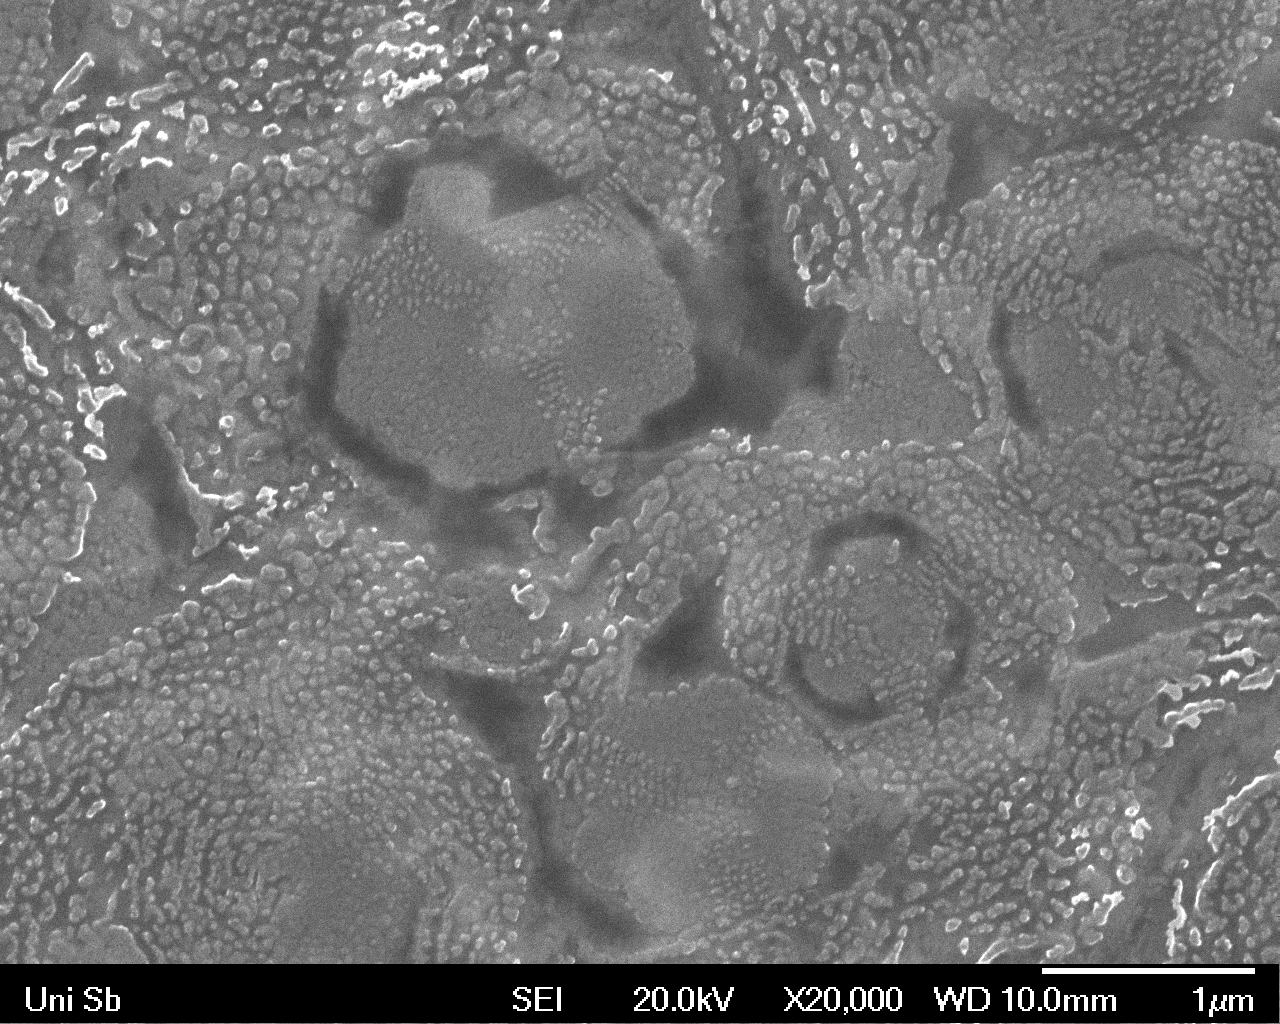
\includegraphics[trim = 0 0 0 0,  clip= true, width = \textwidth]{./pics/am21-sc-7-x20000-1.png}}
			\caption{}\label{subfig::sunken_nd}
		\end{subfigure}
		\hfill
		\begin{subfigure}[t]{ 0.49\linewidth}
			\centering
			\testbox{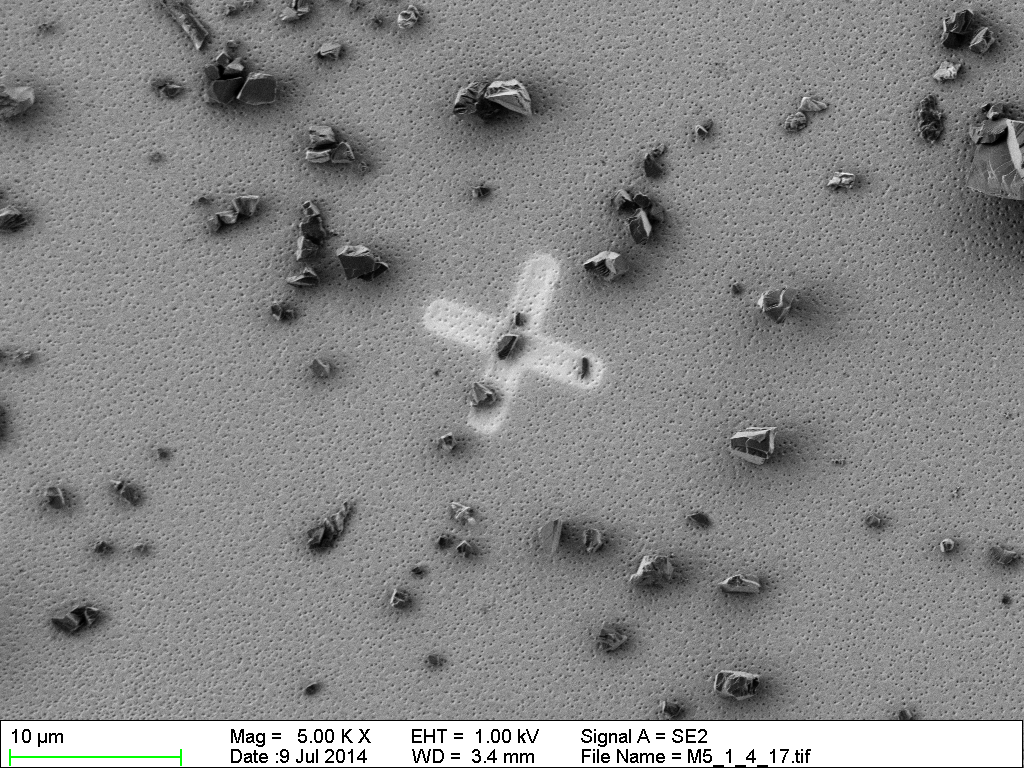
\includegraphics[trim = 0 0 0 0,  clip= true, width = \textwidth]{./pics/M5_1_4_17.png}}
			\caption{}\label{subfig::microdiamonds}
		\end{subfigure}
		\caption{(a) SEM picture of \nds sunken into a \si substrate after annealing at \SI{900}{\celsius} for \SI{3}{h}. Magnification \num{20000}. (b) SEM image of the microdiamonds after milling on an \ir substrate, but before implantation. In the middle of the picture, there is a reference cross milled into the \ir substrate with a focused ion beam. Its size amounts to \SI{10}{\micro\meter}. It can be seen, that the microdiamonds exhibit sizes of a few micrometer.}
		\label{fig::<fig>}
	\end{figure}


	\subsubsection{Final Procedure}\label{subsubsec::final_procedure}

	For the milling process in a vibrational mill, a minimum amount of diamond material is necessary\todo{how much?}.
	When starting with a diamond film, this threshold is easily reached, however, a big quantity of microdiamonds is needed to meet the requirements.
	Therefore, production was carried out at a larger scale after the preliminary tests.
	The microdiamonds were directly spin-coated onto \ir substrates, implanted with \ch{^{28}Si^1+} (implantation energy \SI{900}{keV}, fluence \SI{e11}{\per\centi\meter\squared}) \footnote{Implantation performed by \klug.}
	The microdiamonds were then annealed in vacuum for \SI{3}{\hour} at \SI{900}{\celsius} and oxidized in air for \SI{3}{\hour} at \SI{450}{\celsius}.
	At last, they were milled again to sizes of about \SIlist{40;45;240;260}{nm}.
	The diamonds of sizes \SIlist{40;240}{nm} were annealed in vacuum at \SI{1200}{\celsius}\todo{time?}.









\section{\Ir Substrate}\label{sec::ir_substrate}


\begin{figure}[tp]
	\begin{subfigure}[t]{ 0.49\linewidth}
		\caption{}\label{subfig::wetting}
		\centering
		\testbox{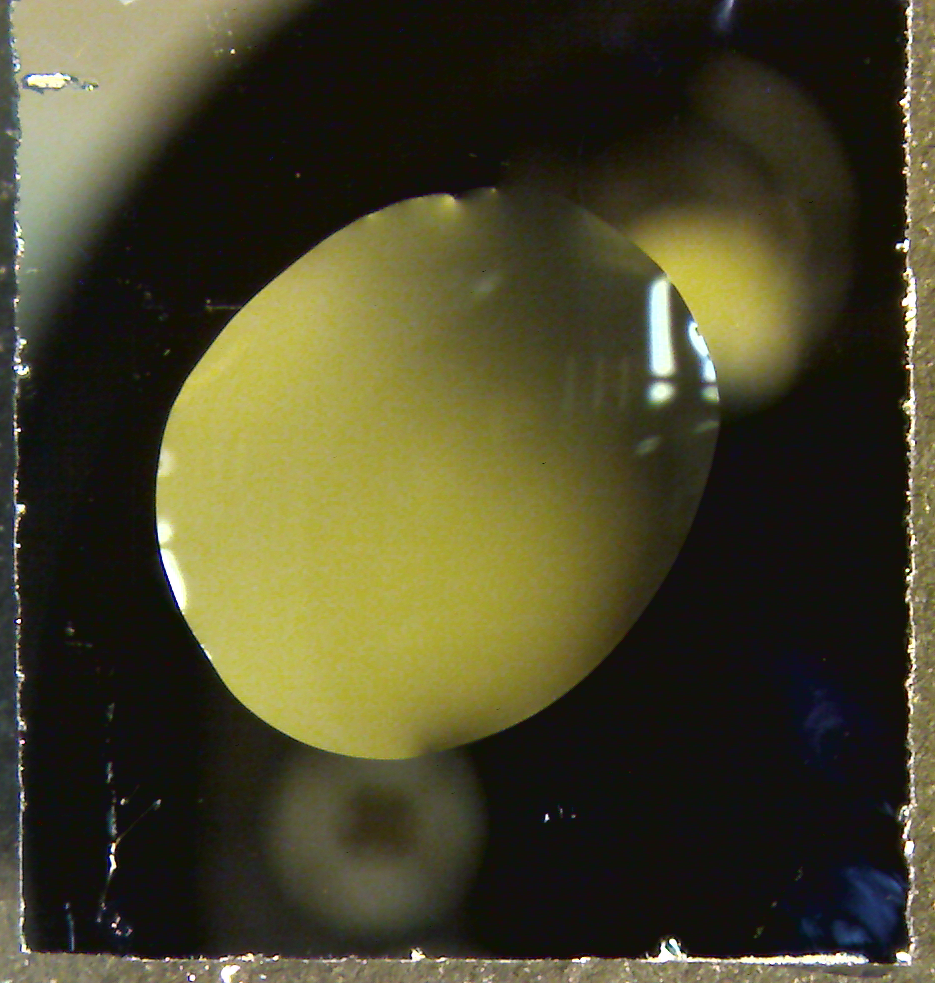
\includegraphics[trim = 0 0 0 0,  clip= true, width = \textwidth]{./pics/benetzung_M11_13_2edit.png}}
	\end{subfigure}
	\hfill
	\begin{subfigure}[t]{ 0.49\linewidth}
		\caption{}\label{subfig::peeled_ir}
		\centering
		\testbox{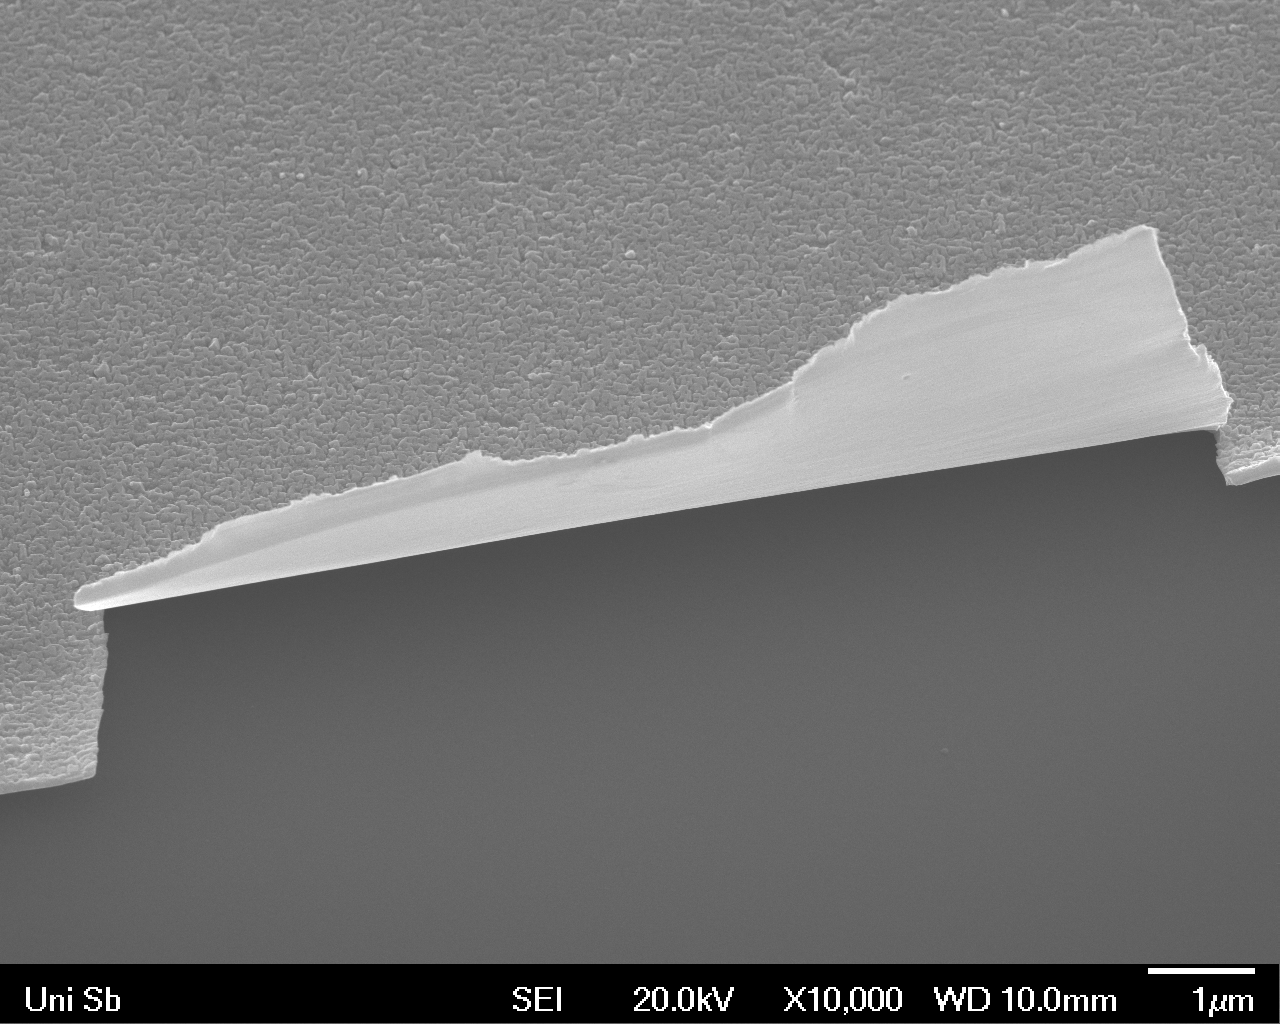
\includegraphics[trim = 0 0 0 0,  clip= true, width = \textwidth]{./pics/siq-basd-siv2-tilt45-x10000-1.png}}
	\end{subfigure}
	\caption{(a) Microcope image of a drop of water on an \ir substrate cleaned with Piranha etch. This picture was used to estimate the contact angle. (b) SEM picture of an \SI{60}{nm} \ir layer that peeled off the substrate after an ultrasonic bath.}
	\label{fig::sem_substrates}
\end{figure}

	As mentioned in \autoref{sec::cvd}, we used a \si substrate with an \ir layer on top for most experiments in order to match the lattice constants of substrate and diamond.
	We also use the same substrates for the experiments with wet-milled diamonds, as using \ir has several advantages:

	\begin{itemize}
		\item The high hydrophilicity of \ir enhances the homogenuity of the nanodiamonds on the substrate after spin-coating or drop-casting.
		The hydrophilicity is further improved by treating the substrate in a Piranha etch (50:50 mixture of sulfuric acid \ch{H2So4} and hydrogen peroxide \ch{H2O2}) by removing oxide layers on the surface.
		The treatment with Piranha etch also has the advantage that all organic contamination is removed.
		Measurements after applying the Piranha cleaning yielded an estimation of the contact angle of slightly more than one degree.
		To determine the contact angle with water, the volume of a water drop is compared to the surface it covers after dropping it onto an \ir substrate, see \autoref{subfig::wetting}.	From that an estimation of the contact angle is deduced.
		\item During the post-processing steps, it is of major importance, that the substrate can withstand high temperatures.
		As described in \autoref{subsubsec::preliminary_tests}, during the preliminary tests with implanted nanodiamonds on a \si substrate we encountered difficulties with diamonds on a \si substrate as the sunk into the surface after annealing.
		In contrast, \ir withstands the high temperatuers required for annealing without damage.
		\item \Ir acts both as a mirror and as an antenna for the \fl light emitted by the \siv \cite{Neu2012a}.
		Therefore, the collection efficiency of the \fl light is enhanced.
	\end{itemize}

	At this point we comment upon a minor complication we experienced when using \ir surfaces.
	If the \ir layer is too thin, it tends to peel off the substrate, see \autoref{subfig::peeled_ir}.
	We encountered this problem during a cleaning procedure in the ultrasonic bath.
	However, this disadvantage is easily circumvented by using a thicker \ir layer.
	For our measurements, we used an \ir layer of a thickness of \SI{130}{nm}, for which we did not encounter any adhesion problems.

	\subsection{Preparation of The Substrate}

	As a preparatory step preceeding drop-casitn, the \ir substrate is cleaned.
	The standard cleaning procedure is comprised of the following cleaning steps in an ultrasonic bath. Each step is in effect for  a duration of \SIrange{3}{7}{\minute}:

	\begin{itemize}
		\item Distilled water with a drop of dishwasher detergent
		\item Isopropanol (\SI{99.9}{\percent} p.a.)
		\item Acetone (\SI{99.9}{\percent} p.a.)
		\item Distilled water
	\end{itemize}

	Thereafter, the substrates are put into a Piranha solution (\SI{50}{\percent} sulfuric acid \ch{H2So4}, \SI{50}{\percent} hydrogen peroxide \ch{H2O2}) to enhance the surface hydrophilicity and therefore obtain a homogeneous distribution of diamonds on the surface.
	They are then put again into distilled water and blow-dried with compressed air to avoid residue from the water.
	The substrates were then either drop-casted or spin-coated with aqueous diamond solutions.
	For the former, the substrates are heated to a temperature of \SI{60}{\celsius} and drops of a volume of about \SI{5}{\micro\liter} are dropped onto the substrate.
	If substantially more than \SI{5}{\micro\liter} is needed, then several drops of about \SI{5}{\micro\liter} are dropped onto the substrate consecutively. A single large drop is ill-advised since the solution would flow off the substrate before drying.
	For spin-coating, a spin coater was build on-site used.
	Here, drops of \SI{5}{\micro\liter} are dropped on the substrate and the spin-coater set to a velocity of \SI{2500}{\rpm} for \SI{3}{\minute}.

 \section{Listing of available samples}

 \begin{table}[tp]
	 \centering
	 \caption[Listing of available wet-milled samples]{Listing of available wet-milled samples. The first column indicates the names of the samples, the second the mean diameter of the \nds, and the third designates how the \si was incorporated into the diamond.} \label{tab::samplenames}
		 \begin{tabular}{llll}
		 \toprule
		 Sample name & Size & Si incorporation & Post-processing \\
		 \midrule
		 \hphtimpfortyfive & \SI{45}{nm} & \textit{implanted} & oxidized in air at \SI{450}{\celsius}\\ \hline
		 \hphtimpeighty & \SI{80}{nm} & \textit{in-situ} & \begin{tabular}[c]{@{}l@{}}annealed in vacuum for \SI{1}{\hour} at \SI{1000}{\celsius}\\ and at \SI{900}{\celsius} for \SI{3}{\hour}\end{tabular}\\ \hline
		 \hphtimptwosixty & \SI{260}{nm} & \textit{in-situ} & oxidized in air at \SI{450}{\celsius}\\ \hline
		 \insituF & \SI{50}{nm} & \textit{in-situ} & \begin{tabular}[c]{@{}l@{}}series of individual samples \\ with diverse post-processing steps\end{tabular}\\ \hline
		 \insituS & \SI{70}{nm} & \textit{in-situ} & \begin{tabular}[c]{@{}l@{}}series of individual samples \\ with diverse post-processing steps\end{tabular}\\ \hline
		 \insituSn & \SI{70}{nm} & \textit{in-situ} &  \begin{tabular}[c]{@{}l@{}}no post-processing \\ subset of \insituS \end{tabular}\\ \hline
		 \insituSo & \SI{70}{nm} & \textit{in-situ} & \begin{tabular}[c]{@{}l@{}}oxidized in air at \SI{450}{\celsius} \\ subset of \insituS \end{tabular}\\ \hline
		 \insituH & \SI{100}{nm} & \textit{in-situ} & \begin{tabular}[c]{@{}l@{}}series of individual samples \\ with diverse post-processing steps\end{tabular}\\ \hline
		 \insituHao & \SI{100}{nm} & \textit{in-situ} & \begin{tabular}[c]{@{}l@{}}annealed in vacuum at \SI{900}{\celsius}, \\ consecutively oxidized in air at \SI{450}{\celsius} \\ subset of \insituH \end{tabular}\\ \hline
		 \implantedTao & \SI{250}{nm} & implanted & \begin{tabular}[c]{@{}l@{}}annealed in vacuum at \SI{900}{\celsius}, \\ consecutively oxidized in air at \SI{450}{\celsius}\end{tabular}\\ \hline
		 \milltwofortyann & \SI{40}{nm} & implanted & \begin{tabular}[c]{@{}l@{}}annealed in vacuum at \SI{1200}{\celsius}, \\  consecutively oxidized in air at \SI{450}{\celsius}\end{tabular}\\ \hline
		 \milltwofiftyno & \SI{50}{nm} & implanted & oxidized in air at \SI{450}{\celsius}\\ \hline
		 \milltwotwofortyann & \SI{240}{nm} & implanted & \begin{tabular}[c]{@{}l@{}}annealed in vacuum at \SI{1200}{\celsius}, \\ consecutively oxidized in air at \SI{450}{\celsius}\end{tabular}\\ \hline
		 \milltwotwosixtyno & \SI{260}{nm} & implanted & oxidized in air at \SI{450}{\celsius}\\
		 \bottomrule
		 \end{tabular}
 \end{table}
